\documentclass{beamer}
\usepackage[utf8]{inputenc}
\usepackage{polski}
% \usepackage[polish]{babel}
\usepackage[T1]{fontenc}
\usepackage{tikz}
\usepackage{tikzducks}
% \usetikzlibrary{decorations.pathmorphing}
\usepackage{multimedia}
\usepackage{graphicx}
\usepackage[justification=centering]{caption}
\usepackage{textcomp}
\usepackage{appendixnumberbeamer}
\usepackage{qrcode}
% \usepackage[natbib, language=polish, sorting=none]{biblatex}
% \addbibresource{lio.bib}
\usepackage{hyperref}
%\usepackage[width=\textwidth]{animate}
%\usepackage{chemformula}
\usepackage{sidecap}
\usepackage{multirow}
\usepackage{rotating}
\usepackage{anyfontsize} % change font size for semposiwko
\usepackage{animate}


\usepackage[natbib, language=polish, sorting=none]{biblatex}
\addbibresource{lio.bib}
\renewcommand*{\bibfont}{\scriptsize}

\usetheme{Szeged}
\usecolortheme{whale}
\setbeamercolor{palette primary}{bg=violet!80!black,fg=white}
\setbeamercolor{palette secondary}{bg=violet!60!black,fg=white}
\setbeamercolor{palette tertiary}{bg=violet!40!black,fg=white}
\setbeamercolor{palette quaternary}{bg=violet!20!black,fg=white}
\setbeamercolor{structure}{fg=violet!60!black}
\setbeamertemplate{caption}{\insertcaption}
% \setbeamertemplate{headline}{
%   \begin{beamercolorbox}[wd=.9\paperwidth]{headline}
%     \vspace{1.5ex}
%     \insertsectionnavigationhorizontal
%     \vspace{1.5ex}
%   \end{beamercolorbox}
% }

\linespread{0.6}

\setbeamertemplate{background}%
{%
    \begin{tikzpicture}[remember picture,overlay]{\node[yshift=1.5cm,xshift=-2cm,opacity=0.1] at (current page.south east)
      {
      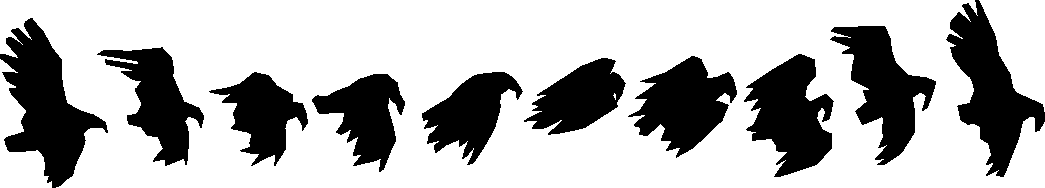
\includegraphics[scale=0.4, angle=20]{ptaki.pdf}
      }
      ;
    \node[yshift=1.0cm,xshift=0.6cm] (logopos) at (current page.south west) {{\begin{tikzpicture}\shuffleducks\duck[signpost=\insertframenumber, \randomhead,scale=.4]\end{tikzpicture}}};
    \pgfmathsetmacro{\progress}{360*(\insertframenumber)/(\inserttotalframenumber)};
    \draw[line width=0.2*3pt] ([xshift=0.55cm] logopos)  arc[radius=0.55cm, start angle=0, end angle=\progress];
    \fill ([shift={(\progress:0.55cm)}] logopos) circle(1pt);

    }
        \end{tikzpicture}
    
}

\newcommand{\SeMPowisko}{%
\large S\normalsize%
\kern-.3em \lower.2ex\hbox{e}%
\lower.2ex\hbox{\large M\normalsize}%
\kern-.1em \raise.1ex\hbox{\large P\normalsize}%
\kern-.3em \lower.2ex\hbox{o}%
\kern-.2em \raise.2ex\hbox{w}%
\lower.2ex\hbox{i}%
s%
\raise.2ex\hbox{k}%
\kern-.3em \lower.2ex\hbox{o}%
}



\title{Materia zabrana z Kosmosu}
% \subtitle{Przegląd niektórych eksperymentów}
\author[M. Winiarski]{Mateusz Winiarski}
\institute[Materia przychodząca z Kosmosu]{fizyka IV$^1$, WFAIS UJ}
\date[today]{Materia przychodząca z kosmosu 2024\\dzisiaj}

\begin{document}

\frame{\titlepage}

\begin{frame}{Spis treści}
    \tableofcontents
\end{frame}

\section{Przeszłość}
\begin{frame}{Jak zdobyć materię kosmiczną?}
    \begin{figure}
        \centering
        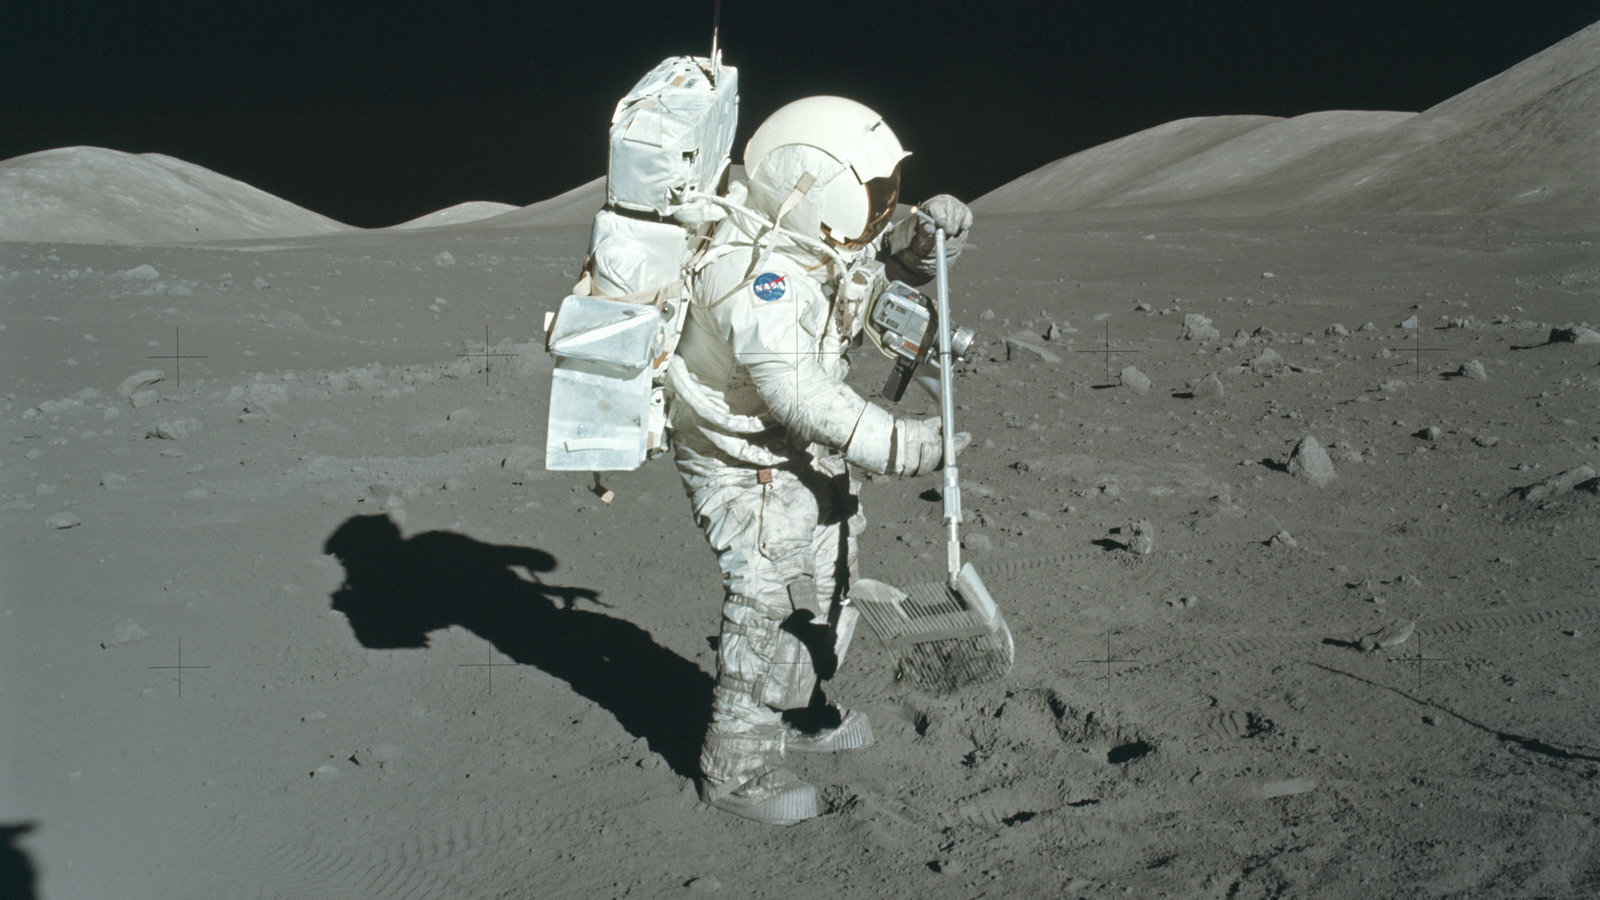
\includegraphics[width=0.75\linewidth]{kosmos/ap17.png}
        \caption{Astronauta misji Apollo 17 z łopatą}
    \end{figure}
\end{frame}

\begin{frame}{Badania materii księżycowej}
    \begin{figure}
        \centering
        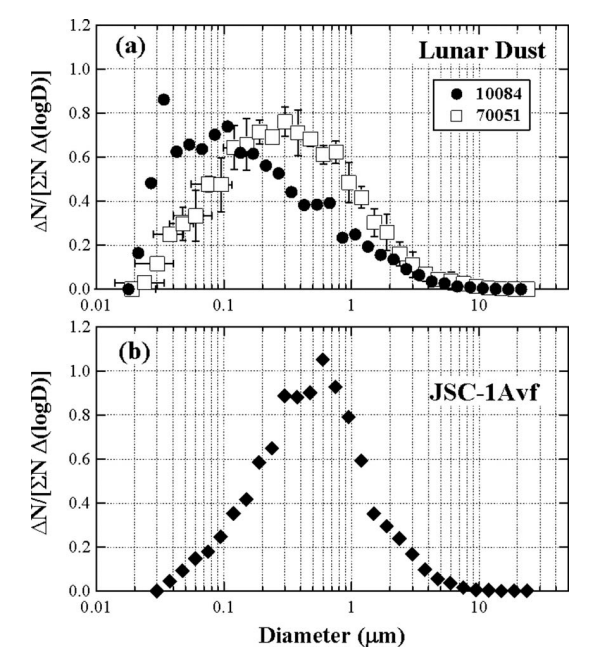
\includegraphics[width=0.5\linewidth]{kosmos/xd.png}
        \caption{Rozkład rozmiaru pyłu księżycowego vs teoria}
    \end{figure}
\end{frame}

\begin{frame}{Zastosowanie pyłu księżycowego}
    \begin{figure}
        \centering
        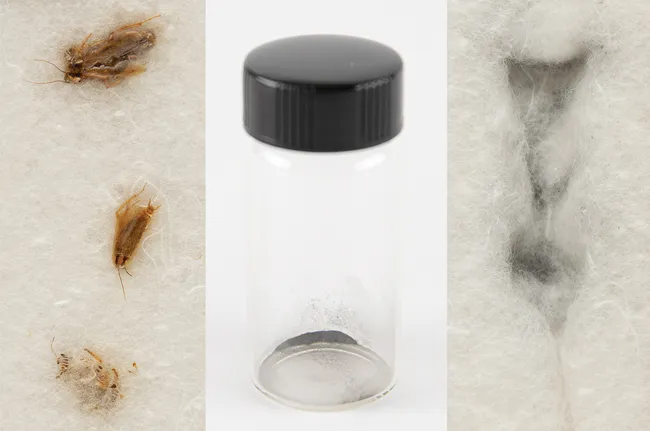
\includegraphics[width=0.75\linewidth]{kosmos/kara.png}
        \caption{Karaluchy i pył księżycowy uzyskany z nich}
    \end{figure}
\end{frame}

\section{Teraźniejszość}

\begin{frame}{Aerożel}
    \begin{figure}
        \centering
        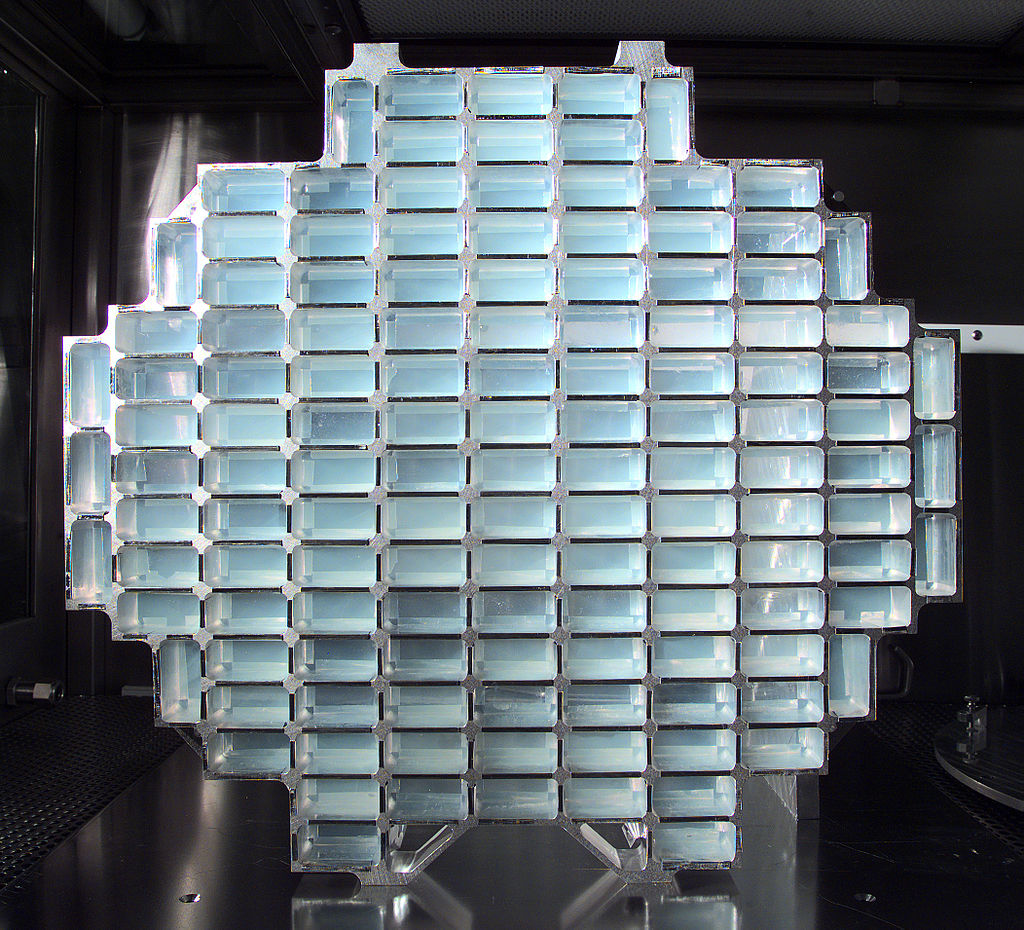
\includegraphics[width=0.5\linewidth]{kosmos/gel.png}
        \caption{Stardust Dust Collector wypełniony aerożelem}
    \end{figure}
\end{frame}

\begin{frame}{Kometa Wild 2}
    \begin{figure}
        \centering
        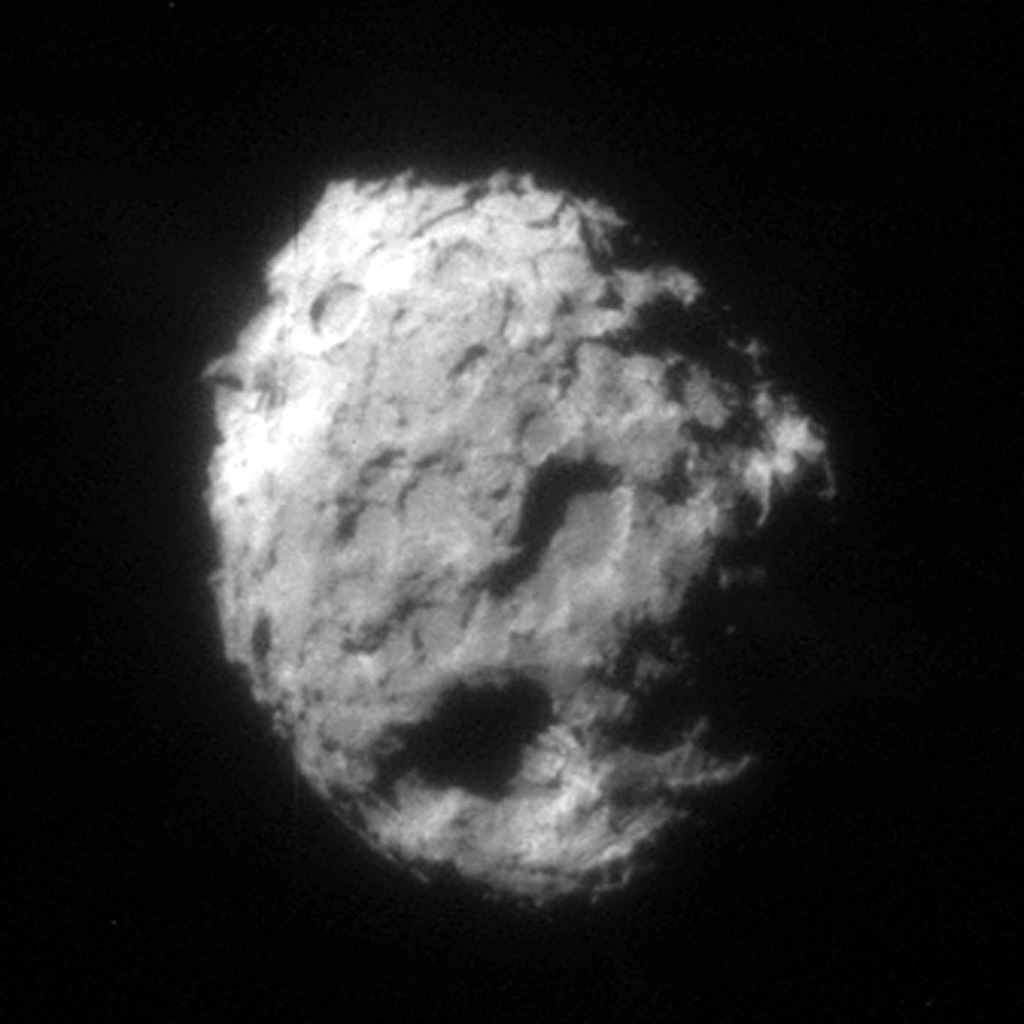
\includegraphics[width=0.5\linewidth]{kosmos/wild.png}
        \caption{Jądro komety Wild 2 widziane 2 stycznia 2004}
    \end{figure}
\end{frame}

\begin{frame}{Cząsteczki komety}
    \begin{figure}
        \centering
        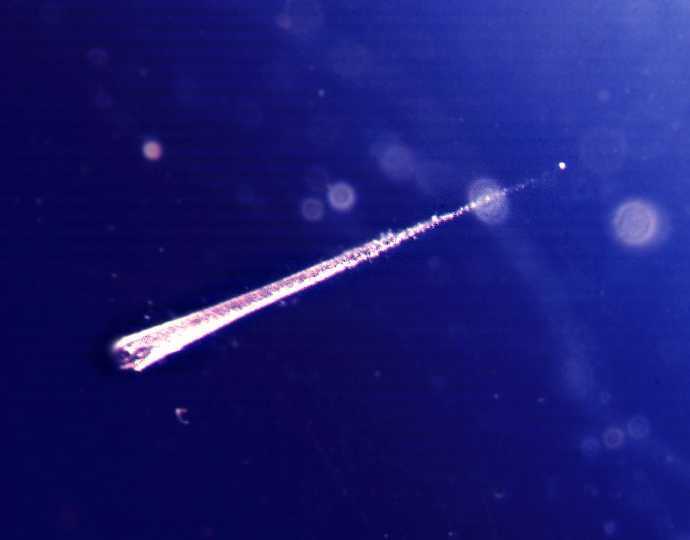
\includegraphics[width=0.75\linewidth]{kosmos/eureca.png}
        \caption{O takie coś}
    \end{figure}
\end{frame}

\begin{frame}{Odkrycia w cząsteczkach komety}
    \begin{figure}
        \centering
        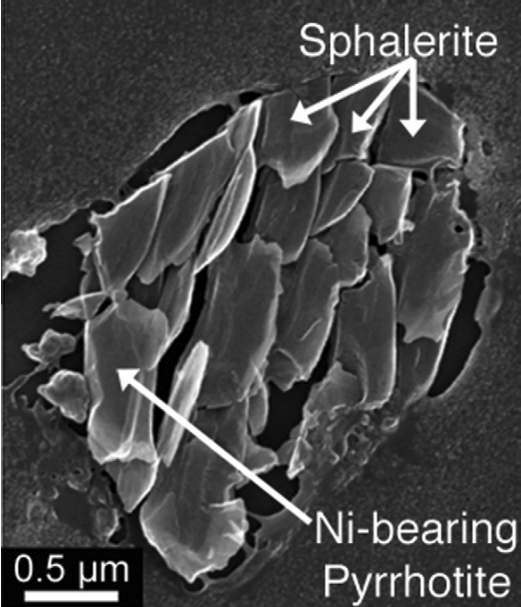
\includegraphics[width=0.5\linewidth]{kosmos/pyrr.png}
        \caption{Obraz TEM cząstki pyłu z komety}
    \end{figure}
\end{frame}

\begin{frame}{Cząsteczki międzygwiezdne}
    \begin{figure}
        \centering
        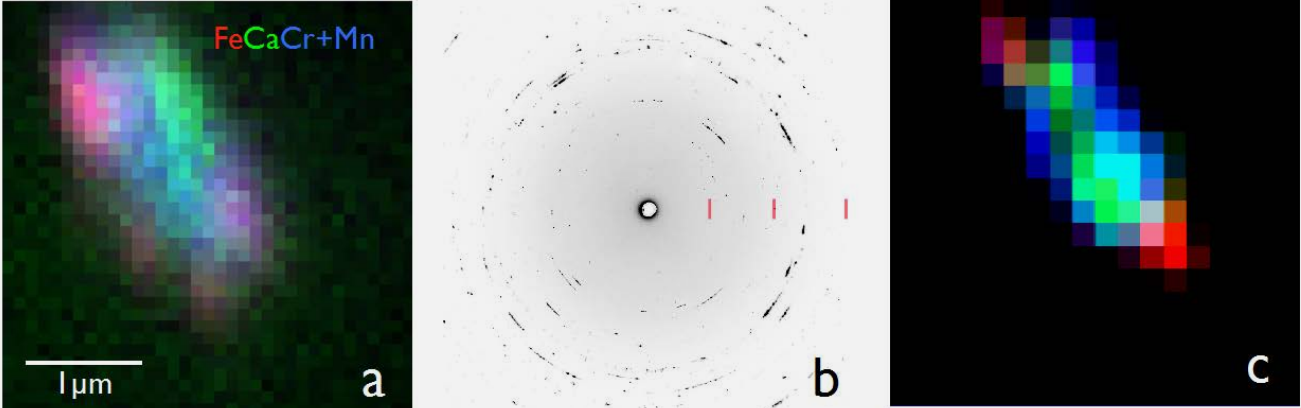
\includegraphics[width=0.99\linewidth]{kosmos/orion.png}
        \caption{XRF, XRD i mapa fazowa cząstki \emph{Orion}}
    \end{figure}
\end{frame}

\begin{frame}{Inne misje I}
    \begin{figure}
        \centering
        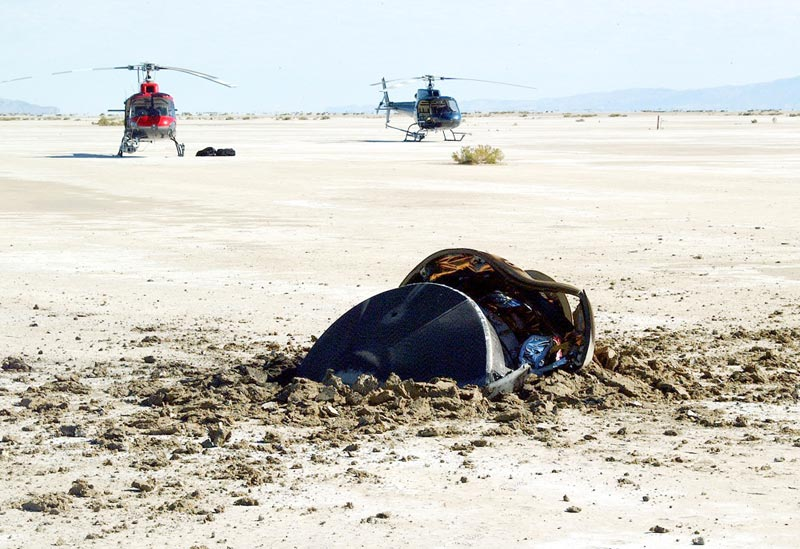
\includegraphics[width=0.75\linewidth]{kosmos/genesis.png}
        \caption{Rozbity lądownik misji Genesis, 5 grudnia 2004}
    \end{figure}
\end{frame}

% \begin{frame}{Inne misje II}
%     \begin{figure}
%         \centering
%         \animategraphics[autoplay,loop,width=0.9\textwidth]{24}{f/frames_}{1}{116}
%         \caption{OSIRIS-REX pobierający próbkę z asteroidy Bennu, 20 października 2020}
%     \end{figure}
% \end{frame}

\section{Przyszłość}
\begin{frame}{Kosmiczne kopalnie}
   \begin{figure}
        \centering
        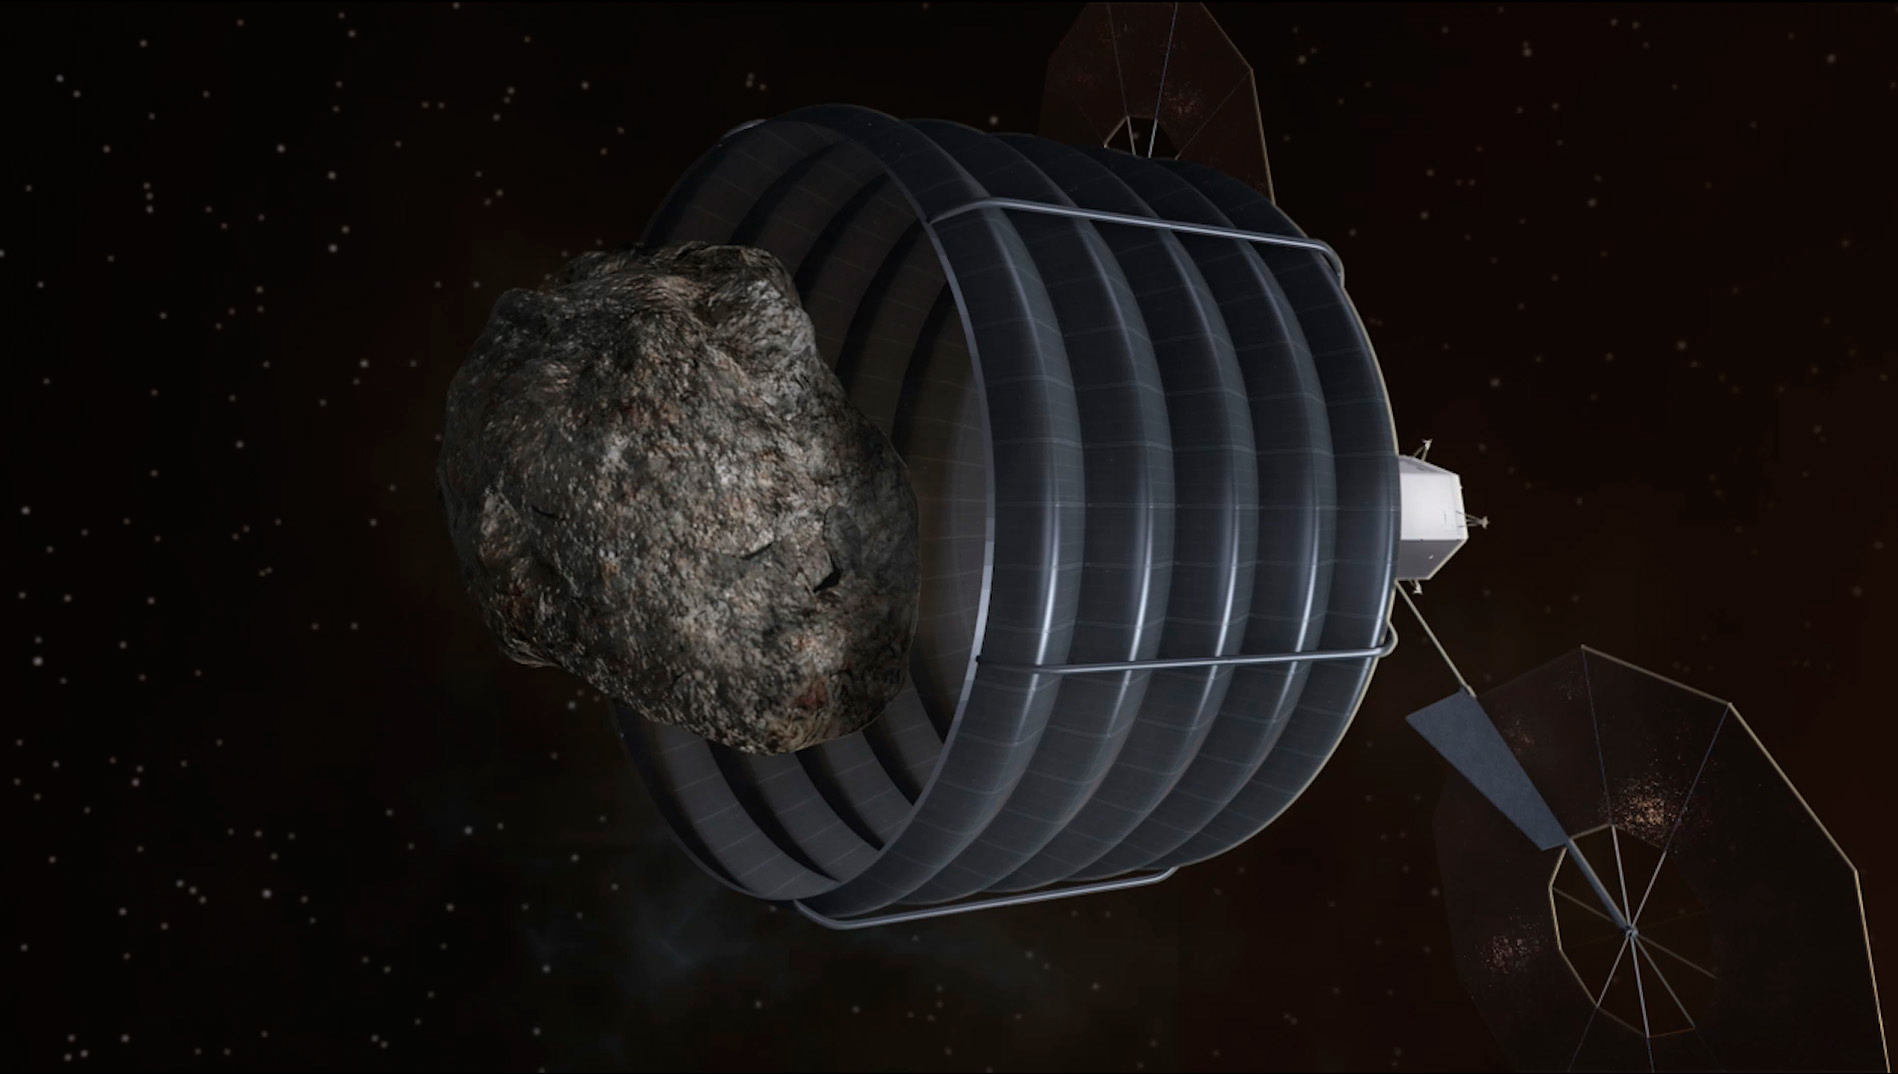
\includegraphics[width=0.75\linewidth]{kosmos/zuodziej.png}
        \caption{Kradnięcie asteroidy}
    \end{figure} 
\end{frame}

\begin{frame}{}

\begin{figure}

\centering
    
\begin{tikzpicture}
      \duck[parrot, body=gray!30!yellow, head=gray!30!yellow, bill=red, torch=gray!70!brown, tshirt=white!90!black, alien=green!50!yellow, ribbon=gray, bowtie=blue!50!black]
      %\addwater{blue!50!cyan}
      \fill[cyan!20!white] (-1.4,1.8) ellipse (1.8 and 0.5);
  \fill[cyan!20!white] (-0.2,1.54) -- (0.2,1.35) -- (0.0,1.6) -- cycle;
	\node at (-1.4,1.8) {Dziynkujã za uwŏgã};
    \end{tikzpicture}
    \end{figure}


    
    \begin{figure}
    \centering
    \qrcode[height=0.3\textwidth]{https://www.overleaf.com/read/xbxgcyvdbwsw}\\
    {\tiny https://www.overleaf.com/read/xbxgcyvdbwsw}

    \end{figure}
\end{frame}

\end{document}
